%************************************************
\chapter{Fundamentals}
\label{chp:fundamentals}
%************************************************

This chapter introduces the (truly simple) basic notions of \arsclassica{} and presents its fundamental ideas and distinctive features.


\section{Introduction}

The \arsclassica{} package changes some typographical features of the \classicthesis{} style, designed by Andr\'e Miede~\citep{miede:classicthesis,pantieri:classicthesis}. It allows to reproduce the layout of the \LaTeX{} guide \emph{The Art of Writing with \LaTeX}~\citep{pantieri:art} (in Italian) and of this document. The hint for this original reworking of \classicthesis{} was given to me by Daniel Gottschlag.



\section{Use of the package}

This package is shaped to be executed on a \emph{complete} installation of \miktex{} or \texlive, and uses freely available fonts.
It works with the \clsname{KOMA-Script} classes (\clsname{scrreprt}, \clsname{scrbook} and \clsname{scrartcl}) and requires the \pkgname{classicthesis} package, \emph{updated to the last version available (the~4.0)}. \arsclassica{} must be loaded \emph{after} \pkgname{classicthesis}:
\begin{code}
\document£**£class[£*\meta{\dots\unkern}*£]{scrreprt} % or scrbook or scrartcl

\usepackage[£*\meta{\dots\unkern}*£]{classicthesis}
\usepackage{arsclassica}

\begin{document}
£*\dots*£
\end{document}
\end{code}

For example, this document has been produced with the following code:
\begin{code}
\document£**£class[10pt,a4paper,twoside,openright,titlepage,fleqn,%
               headinclude,footinclude,BCOR5mm,%
               numbers=noenddot,cleardoublepage=empty,%
               tablecaptionabove]{scrreprt}

\usepackage{£*\meta{\dots\unkern}*£}
\usepackage{subfig}
\usepackage[eulerchapternumbers,subfig,beramono,%
            eulermath,pdfspacing]{classicthesis}
\usepackage{arsclassica}

\begin{document}
£*\dots*£
\end{document}
\end{code}

It is recommended, but not compulsory, to use the options \optname{beramono}, \optname{eulerchapternumbers} and \optname{eulermath} together with \arsclassica.






\section{The style}

The typographical style achieved with \arsclassica{} differs from ClassicThesis in the following points:
\begin{itemize}
\item use of Iwona\index{Iwona} font, by Janusz M.~Nowacki, for the titles of the sectioning units of the document (chapters, sections, subsections, sub-subsections, paragraphs and subparagraphs), for the labels of description lists, for the headlines and the label of the captions (\classicthesis{} does not use any sans serif font);
\item customized chapter numbers;
\item semi-transparent headlines; the headlines are separated from the page number by a small rule;
\item captions with labels in boldface (\classicthesis{} does not use any boldface font);
\item itemize lists with semi-transparent bullets.
\end{itemize}

The \arsclassica{} package is designed  to provide a ready-to-use typographical style: therefore it has no loading option and it is \emph{not} configurable or customizable in any way. If you change the previous settings, you will risk to destroy the balance of the style, so it is \emph{highly recommended} to keep them unchanged.

One of the principles of \LaTeX{} is that it allows the author to take no interest in the typographical questions, permitting him to focus only the structure and the contents of the document. This fact should always be taken in consideration: using a style written by others, the user accepts all the typographical settings chosen for him by the author of the style, and he is not forced to study typography to fix the layout of his publications. This is the case of \arsclassica{} too: if you change its settings, you will deny this philosophy and, consequently, you must study (a lot of) typography to achieve acceptable results. 

The style achieved with \arsclassica{} is \emph{not} therefore configurable or customizable. The typographical style is something of very personal: if you like the package and find attractive the idea to take no interest in the problem of the style definition, then you will use \arsclassica{} with satisfaction; otherwise, if you have different needs or you are not satisfied with the layout of the package, then you should try other classes or packages, even building your own style.



\section{New commands}

The package offers the \cmdname{ctLaTeX}, \cmdname{ctLaTeXe} and \cmdname{ctTeX} commands, which allow to reproduce respectively the \LaTeX, \LaTeXe{} and \TeX{} logos correctly written in Iwona.\index{Iwona}






\section{Examples}

\begin{figure}
\centering
\subfloat[Asia personas duo.]
{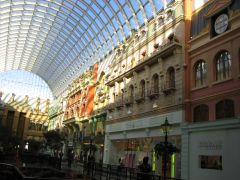
\includegraphics[width=.45\columnwidth]{Example_1}} \quad
\subfloat[Pan ma signo.]
{\label{fig:example-b}%
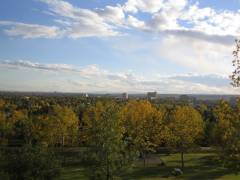
\includegraphics[width=.45\columnwidth]{Example_2}} \\
\subfloat[Methodicamente o uno.]
{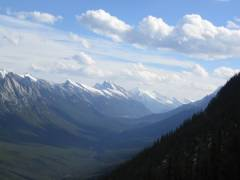
\includegraphics[width=.45\columnwidth]{Example_3}} \quad
\subfloat[Titulo debitas.]
{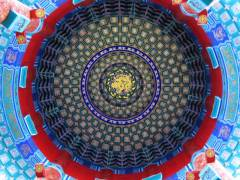
\includegraphics[width=.45\columnwidth]{Example_4}}
\caption[Tu duo titulo debitas latente.]{Tu duo titulo debitas
latente.}\label{fig:example}
\end{figure}

Note: The content of this chapter is just some dummy text. It is not a real language.

Lorem ipsum dolor sit amet, consectetuer adipiscing elit. Ut purus elit, vestibulum ut, placerat ac, adipiscing vitae, felis. Curabitur dictum gravida mauris. Nam arcu libero, nonummy eget, consectetuer id, vulputate a, magna. Donec vehicula augue eu neque.

\subsection*{A subsection}
\lipsum[2]

\subsubsection*{A sub-subsection}
\lipsum[3]

\paragraph{A paragraph} Lorem ipsum dolor sit amet, consectetuer adipiscing elit. Ut purus elit, vestibulum ut, placerat ac, adipiscing vitae, felis. Curabitur dictum gravida mauris. Nam arcu libero, nonummy eget, consectetuer id, vulputate a, magna.

\bigskip

\lipsum[2]

\begin{description}
\item[Mane] Lorem ipsum dolor sit amet, consectetuer adipiscing elit. 
\item[Tekel] Ut purus elit, vestibulum ut, placerat ac, adipiscing vitae, felis. Curabitur dictum gravida mauris.
\item[Fares] Nam arcu libero, nonummy eget, consectetuer 
id, vulputate a, magna.
\end{description}

\begin{table}
\caption[Lorem ipsum dolor.]{Lorem ipsum dolor sit amet.}
\centering
\begin{tabular}{cc}
\toprule
$p$ & $\lnot p$ \\ 
\midrule
V   & F \\ 
F   & V \\
\bottomrule 
\end{tabular}
\end{table}

\lipsum[1]




